\documentclass[review]{elsarticle} %review=doublespace preprint=single 5p=2 column
%%% Begin My package additions %%%%%%%%%%%%%%%%%%%
\usepackage[hyphens]{url}

  \journal{An awesome journal} % Sets Journal name


\usepackage{lineno} % add
\providecommand{\tightlist}{%
  \setlength{\itemsep}{0pt}\setlength{\parskip}{0pt}}

\usepackage{graphicx}
%%%%%%%%%%%%%%%% end my additions to header

\usepackage[T1]{fontenc}
\usepackage{lmodern}
\usepackage{amssymb,amsmath}
\usepackage{ifxetex,ifluatex}
\usepackage{fixltx2e} % provides \textsubscript
% use upquote if available, for straight quotes in verbatim environments
\IfFileExists{upquote.sty}{\usepackage{upquote}}{}
\ifnum 0\ifxetex 1\fi\ifluatex 1\fi=0 % if pdftex
  \usepackage[utf8]{inputenc}
\else % if luatex or xelatex
  \usepackage{fontspec}
  \ifxetex
    \usepackage{xltxtra,xunicode}
  \fi
  \defaultfontfeatures{Mapping=tex-text,Scale=MatchLowercase}
  \newcommand{\euro}{€}
\fi
% use microtype if available
\IfFileExists{microtype.sty}{\usepackage{microtype}}{}
\bibliographystyle{elsarticle-harv}
\usepackage{color}
\usepackage{fancyvrb}
\newcommand{\VerbBar}{|}
\newcommand{\VERB}{\Verb[commandchars=\\\{\}]}
\DefineVerbatimEnvironment{Highlighting}{Verbatim}{commandchars=\\\{\}}
% Add ',fontsize=\small' for more characters per line
\usepackage{framed}
\definecolor{shadecolor}{RGB}{248,248,248}
\newenvironment{Shaded}{\begin{snugshade}}{\end{snugshade}}
\newcommand{\KeywordTok}[1]{\textcolor[rgb]{0.13,0.29,0.53}{\textbf{#1}}}
\newcommand{\DataTypeTok}[1]{\textcolor[rgb]{0.13,0.29,0.53}{#1}}
\newcommand{\DecValTok}[1]{\textcolor[rgb]{0.00,0.00,0.81}{#1}}
\newcommand{\BaseNTok}[1]{\textcolor[rgb]{0.00,0.00,0.81}{#1}}
\newcommand{\FloatTok}[1]{\textcolor[rgb]{0.00,0.00,0.81}{#1}}
\newcommand{\ConstantTok}[1]{\textcolor[rgb]{0.00,0.00,0.00}{#1}}
\newcommand{\CharTok}[1]{\textcolor[rgb]{0.31,0.60,0.02}{#1}}
\newcommand{\SpecialCharTok}[1]{\textcolor[rgb]{0.00,0.00,0.00}{#1}}
\newcommand{\StringTok}[1]{\textcolor[rgb]{0.31,0.60,0.02}{#1}}
\newcommand{\VerbatimStringTok}[1]{\textcolor[rgb]{0.31,0.60,0.02}{#1}}
\newcommand{\SpecialStringTok}[1]{\textcolor[rgb]{0.31,0.60,0.02}{#1}}
\newcommand{\ImportTok}[1]{#1}
\newcommand{\CommentTok}[1]{\textcolor[rgb]{0.56,0.35,0.01}{\textit{#1}}}
\newcommand{\DocumentationTok}[1]{\textcolor[rgb]{0.56,0.35,0.01}{\textbf{\textit{#1}}}}
\newcommand{\AnnotationTok}[1]{\textcolor[rgb]{0.56,0.35,0.01}{\textbf{\textit{#1}}}}
\newcommand{\CommentVarTok}[1]{\textcolor[rgb]{0.56,0.35,0.01}{\textbf{\textit{#1}}}}
\newcommand{\OtherTok}[1]{\textcolor[rgb]{0.56,0.35,0.01}{#1}}
\newcommand{\FunctionTok}[1]{\textcolor[rgb]{0.00,0.00,0.00}{#1}}
\newcommand{\VariableTok}[1]{\textcolor[rgb]{0.00,0.00,0.00}{#1}}
\newcommand{\ControlFlowTok}[1]{\textcolor[rgb]{0.13,0.29,0.53}{\textbf{#1}}}
\newcommand{\OperatorTok}[1]{\textcolor[rgb]{0.81,0.36,0.00}{\textbf{#1}}}
\newcommand{\BuiltInTok}[1]{#1}
\newcommand{\ExtensionTok}[1]{#1}
\newcommand{\PreprocessorTok}[1]{\textcolor[rgb]{0.56,0.35,0.01}{\textit{#1}}}
\newcommand{\AttributeTok}[1]{\textcolor[rgb]{0.77,0.63,0.00}{#1}}
\newcommand{\RegionMarkerTok}[1]{#1}
\newcommand{\InformationTok}[1]{\textcolor[rgb]{0.56,0.35,0.01}{\textbf{\textit{#1}}}}
\newcommand{\WarningTok}[1]{\textcolor[rgb]{0.56,0.35,0.01}{\textbf{\textit{#1}}}}
\newcommand{\AlertTok}[1]{\textcolor[rgb]{0.94,0.16,0.16}{#1}}
\newcommand{\ErrorTok}[1]{\textcolor[rgb]{0.64,0.00,0.00}{\textbf{#1}}}
\newcommand{\NormalTok}[1]{#1}
\usepackage{longtable,booktabs,array}
\usepackage{calc} % for calculating minipage widths
% Correct order of tables after \paragraph or \subparagraph
\usepackage{etoolbox}
\makeatletter
\patchcmd\longtable{\par}{\if@noskipsec\mbox{}\fi\par}{}{}
\makeatother
% Allow footnotes in longtable head/foot
\IfFileExists{footnotehyper.sty}{\usepackage{footnotehyper}}{\usepackage{footnote}}
\makesavenoteenv{longtable}
\ifxetex
  \usepackage[setpagesize=false, % page size defined by xetex
              unicode=false, % unicode breaks when used with xetex
              xetex]{hyperref}
\else
  \usepackage[unicode=true]{hyperref}
\fi
\hypersetup{breaklinks=true,
            bookmarks=true,
            pdfauthor={},
            pdftitle={Article Name},
            colorlinks=true,
            urlcolor=blue,
            linkcolor=blue,
            pdfborder={0 0 0}}
\urlstyle{same}  % don't use monospace font for urls

\setcounter{secnumdepth}{5}
% Pandoc toggle for numbering sections (defaults to be off)

% Pandoc citation processing

% Pandoc header
% nullify the abstract environment
% \renewenvironment{abstract}{}{}

% Use the `align` environment inside the `subequations` environment 
% from the `amsmath` package to label equation with subnumber (e.g. 1a, 1b)
\usepackage{amsmath}

%fix position of table, figure
\usepackage{float}
\let\origfigure\figure
\let\endorigfigure\endfigure
\renewenvironment{figure}[1][2] {
    \expandafter\origfigure\expandafter[H]
} {
    \endorigfigure
}
\usepackage{booktabs}
\usepackage{longtable}
\usepackage{array}
\usepackage{multirow}
\usepackage{wrapfig}
\usepackage{float}
\usepackage{colortbl}
\usepackage{pdflscape}
\usepackage{tabu}
\usepackage{threeparttable}
\usepackage{threeparttablex}
\usepackage[normalem]{ulem}
\usepackage{makecell}
\usepackage{xcolor}



\begin{document}
\begin{frontmatter}

  \title{Article Name}
    \author[a,1]{Author One}
   \ead{one@example.com} 
    \author[a,b]{Author Two\corref{1}}
   \ead{two@example.com} 
    \author[c]{Author Three\corref{2}}
   \ead{three@example.com} 
    \author[a]{Author Four\corref{2}}
   \ead{four@example.com} 
      \address[a]{Graduate School of Engineering, Nagasaki University, 1-14 Bunkyo-machi,
Nagasaki 852-8521, Japan}
    \address[b]{Department, University, Street, City, State, Zip}
    \address[c]{Department, University, Street, City, State, Zip}
      \cortext[1]{Corresponding Author}
    \cortext[2]{Equal contribution}
    \cortext[]{\textsuperscript{1}Present address: Department, University, Street,
City, State, Zip}
  
  \begin{abstract}
  This is the abstract.\\
  1. what is the study about?\\
  2. what problem does it address?\\
  3. how did you conduct the research?\\
  4. what were the main findings?\\
  5. why is it important?
  \end{abstract}
   \begin{keyword} keywordA, keywordB\end{keyword}
 \end{frontmatter}

\newpage

\section{Introduction}\label{intro}

Setting \textbf{global options} that apply to every chunk in the file.

\begin{Shaded}
\begin{Highlighting}[]
\NormalTok{```\{r setup, include=FALSE\}}
\NormalTok{knitr::opts_chunk$set(echo = FALSE, message = FALSE, warning = FALSE)}

\NormalTok{library(here)}
\NormalTok{library(tidyverse)}
\NormalTok{library(kableExtra)}

\FunctionTok{# displaying 20000 instead of 2 x 10^4}
\NormalTok{options(scipen = 999)}
\NormalTok{```}
\end{Highlighting}
\end{Shaded}

\begin{Shaded}
\begin{Highlighting}[]
\NormalTok{```\{r\}}
\FunctionTok{# import data}
\NormalTok{data <- read_csv(here("data", "process", "newdata.csv"))}
\NormalTok{```}
\end{Highlighting}
\end{Shaded}

Ordered list items:

\begin{Shaded}
\begin{Highlighting}[]
\NormalTok{1. }\FloatTok{general information}
\FloatTok{1. research gap}
\FloatTok{1. research aim}
\end{Highlighting}
\end{Shaded}

The output is:

\begin{enumerate}
\def\labelenumi{\arabic{enumi}.}
\tightlist
\item
  general information
\item
  research gap
\item
  research aim
\end{enumerate}

\section{Materials and methods}\label{method}

\subsection{Adding figures}\label{figure}

Add Fig. \ref{fig:boxplot} here.

\begin{Shaded}
\begin{Highlighting}[]
\NormalTok{```\{r boxplot, fig.cap='A boxplot', out.height="50%", fig.align='center'\}}
\NormalTok{knitr::include_graphics(here::here("results", "figures", "boxplot.pdf"))}
\NormalTok{```}
\end{Highlighting}
\end{Shaded}

\begin{figure}

{\centering 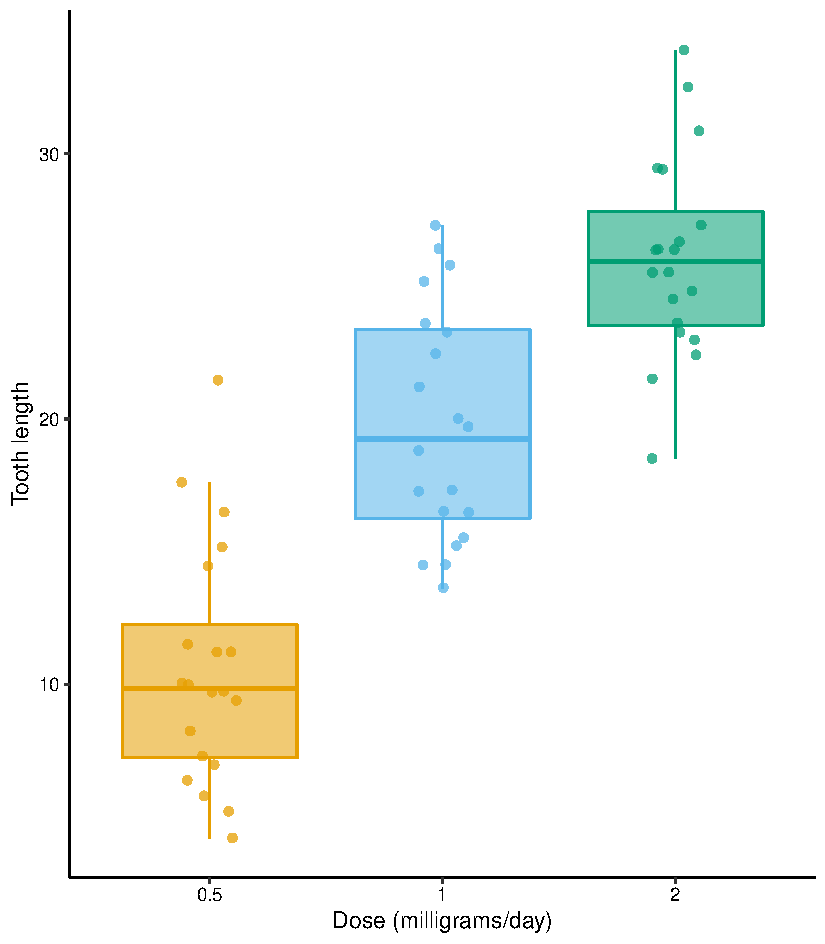
\includegraphics[height=0.5\textheight]{C:/Users/LY/Google Drive/Git/writing_journal_article_in_rmarkdown/results/figures/boxplot} 

}

\caption{A boxplot}\label{fig:boxplot}
\end{figure}

If the caption is too long (Fig. \ref{fig:2021}), use
\href{https://bookdown.org/yihui/rmarkdown/bookdown-markdown.html\#text-references}{text-reference}.

\texttt{(ref:longcaption)\ This\ is\ a\ very\ long\ caption}

\begin{Shaded}
\begin{Highlighting}[]
\NormalTok{```\{r 2021, fig.cap='(ref:longcaption', out.width="50%", fig.align='center'\}}
\NormalTok{knitr::include_graphics(here::here("results", "pictures", "2021.png"))}
\NormalTok{```}
\end{Highlighting}
\end{Shaded}



\begin{figure}

{\centering 
\includegraphics[width=0.5\linewidth]{C:/Users/LY/Google Drive/Git/writing_journal_article_in_rmarkdown/results/pictures/2021} 

}

\caption{This is a very long caption}\label{fig:2021}
\end{figure}

\subsection{Adding tables}\label{table}

\begin{Shaded}
\begin{Highlighting}[]
\NormalTok{```\{r table1\}}
\NormalTok{data %>% }
\BaseNTok{          group_by(supp) %>%}
\BaseNTok{          summarise(median = median(len),}
\BaseNTok{                    mean = mean(len)) %>% }
\BaseNTok{    kable("latex",}
\BaseNTok{          booktabs = T,}
\BaseNTok{          col.names = c("Supplement type", }
\BaseNTok{                    "Median",}
\BaseNTok{                    "Mean"), }
\BaseNTok{          align = "cll",}
\BaseNTok{          caption = "\textbackslash{}\textbackslash{}label\{tab:cooltable\}Mean and Median")}
\NormalTok{```}
\end{Highlighting}
\end{Shaded}

\begin{table}

\caption{\label{tab:unnamed-chunk-2}\label{tab:cooltable}Mean and Median}
\centering
\begin{tabular}[t]{cll}
\toprule
Supplement type & Median & Mean\\
\midrule
OJ & 22.7 & 20.66333\\
VC & 16.5 & 16.96333\\
\bottomrule
\end{tabular}
\end{table}

\begin{Shaded}
\begin{Highlighting}[]
\NormalTok{```\{r table2\}}
\NormalTok{para = c("Intercept ($\textbackslash{}\textbackslash{}beta_0$)",}
\BaseNTok{         "Parameter 1 ($\textbackslash{}\textbackslash{}beta_1$)",}
\BaseNTok{         "Parameter 2 ($\textbackslash{}\textbackslash{}beta_2$)",}
\BaseNTok{         "Hurdle probability ($\textbackslash{}\textbackslash{}theta$)")}

\NormalTok{tab <- data.frame(}
\BaseNTok{    Parameter = para,}
\BaseNTok{    Estimate = c(1.6, 1.2, 6.2, 0.5),}
\BaseNTok{    Error = c(0.41, 0.02, 0.09, 0.07),}
\BaseNTok{    CI = c("[0.698, 2.477]",}
\BaseNTok{           "[1.123, 1.235]",}
\BaseNTok{           "[6.051, 6.423]",}
\BaseNTok{           "[0.353, 0.644]"),}
\BaseNTok{    Rhat = c(rep("1.00", 4)))}

\NormalTok{kable(tab,}
\BaseNTok{      "latex",}
\BaseNTok{      align = "lcccc",}
\BaseNTok{      booktabs = TRUE,}
\BaseNTok{      escape = FALSE,}
\BaseNTok{      caption = "\textbackslash{}\textbackslash{}label\{tab:mathtable\}A table with LaTeX Math symbols")}
\NormalTok{```}
\end{Highlighting}
\end{Shaded}

\begin{table}

\caption{\label{tab:unnamed-chunk-3}\label{tab:mathtable}A table with LaTeX Math symbols}
\centering
\begin{tabular}[t]{lcccc}
\toprule
Parameter & Estimate & Error & CI & Rhat\\
\midrule
Intercept ($\beta_0$) & 1.6 & 0.41 & {}[0.698, 2.477] & 1.00\\
Parameter 1 ($\beta_1$) & 1.2 & 0.02 & {}[1.123, 1.235] & 1.00\\
Parameter 2 ($\beta_2$) & 6.2 & 0.09 & {}[6.051, 6.423] & 1.00\\
Hurdle probability ($\theta$) & 0.5 & 0.07 & {}[0.353, 0.644] & 1.00\\
\bottomrule
\end{tabular}
\end{table}

\subsection{Adding equation}\label{equation}

\begin{Shaded}
\begin{Highlighting}[]
\NormalTok{1. }\FloatTok{The _variable_ \textbackslash{}(x\textbackslash{}) and the __function__ \textbackslash{}(f(x)\textbackslash{})}
\FloatTok{1. The *variable* $x$ and the **function** $f(x)$}
\FloatTok{1. superscript^2^}
\FloatTok{1. NO~2~, NO~3~, PO~4~, NH~4~}
\FloatTok{1. 25 µL}
\end{Highlighting}
\end{Shaded}

The output is:

\begin{enumerate}
\def\labelenumi{\arabic{enumi}.}
\tightlist
\item
  The \emph{variable} \(x\) and the \textbf{function} \(f(x)\)
\item
  The \emph{variable} \(x\) and the \textbf{function} \(f(x)\)
\item
  superscript\textsuperscript{2}
\item
  NO\textsubscript{2}, NO\textsubscript{3}, PO\textsubscript{4},
  NH\textsubscript{4}
\item
  25 µL
\end{enumerate}

Adding equations using the LaTeX syntax

\begin{Shaded}
\begin{Highlighting}[]
\SpecialStringTok{\textbackslash{}[Y|X }\SpecialCharTok{\textbackslash{}sim}\SpecialStringTok{ Bernoulli(p)\textbackslash{}]}
\end{Highlighting}
\end{Shaded}

\[Y|X \sim Bernoulli(p)\]

\begin{Shaded}
\begin{Highlighting}[]
\KeywordTok{\textbackslash{}begin}\NormalTok{\{}\ExtensionTok{equation}\NormalTok{\}}
\SpecialCharTok{\textbackslash{}label}\SpecialStringTok{\{eq:cutoff\}}
\SpecialStringTok{p(x) = P(Y = 1|X = x) = }
\SpecialCharTok{\textbackslash{}left\textbackslash{}\{}
\SpecialStringTok{    }\KeywordTok{\textbackslash{}begin}\NormalTok{\{}\ExtensionTok{array}\NormalTok{\}}\SpecialStringTok{\{lr\}}
\SpecialStringTok{          p_1 = P(Y = 1|X }\SpecialCharTok{\textbackslash{}le}\SpecialStringTok{ cp), & }\SpecialCharTok{\textbackslash{}text}\NormalTok{\{if \}}\SpecialStringTok{ x }\SpecialCharTok{\textbackslash{}le}\SpecialStringTok{ cp}\SpecialCharTok{\textbackslash{}\textbackslash{}}
\SpecialStringTok{          p_2 = P(Y = 1|X > cp), & }\SpecialCharTok{\textbackslash{}text}\NormalTok{\{if \}}\SpecialStringTok{ x > cp}
\SpecialStringTok{    }\KeywordTok{\textbackslash{}end}\NormalTok{\{}\SpecialStringTok{array\}}
\SpecialCharTok{\textbackslash{}right}\SpecialStringTok{.}
\KeywordTok{\textbackslash{}end}\NormalTok{\{}\ExtensionTok{equation}\NormalTok{\}}
\end{Highlighting}
\end{Shaded}

\begin{equation}
\label{eq:cutoff}
p(x) = P(Y = 1|X = x) = 
\left\{
    \begin{array}{lr}
          p_1 = P(Y = 1|X \le cp), & \text{if } x \le cp\\
          p_2 = P(Y = 1|X > cp), & \text{if } x > cp
    \end{array}
\right.
\end{equation}

\begin{Shaded}
\begin{Highlighting}[]
\KeywordTok{\textbackslash{}begin}\NormalTok{\{}\ExtensionTok{subequations}\NormalTok{\}}
  \KeywordTok{\textbackslash{}label}\NormalTok{\{}\ExtensionTok{eq:model}\NormalTok{\}}
  \KeywordTok{\textbackslash{}begin}\NormalTok{\{}\ExtensionTok{align}\NormalTok{\}}
\SpecialStringTok{  }\SpecialCharTok{\textbackslash{}label}\SpecialStringTok{\{eq:modela\}}
\SpecialStringTok{P(y|}\SpecialCharTok{\textbackslash{}theta}\SpecialStringTok{, }\SpecialCharTok{\textbackslash{}lambda}\SpecialStringTok{) = }
\SpecialCharTok{\textbackslash{}left\textbackslash{}\{}
\SpecialStringTok{    }\KeywordTok{\textbackslash{}begin}\NormalTok{\{}\ExtensionTok{array}\NormalTok{\}}\SpecialStringTok{\{lr\}}
\SpecialStringTok{       }\SpecialCharTok{\textbackslash{}theta}\SpecialStringTok{ & }\SpecialCharTok{\textbackslash{}text}\NormalTok{\{if \}}\SpecialStringTok{ y = 0}\SpecialCharTok{\textbackslash{}\textbackslash{}}
\SpecialStringTok{       (1 - }\SpecialCharTok{\textbackslash{}theta}\SpecialStringTok{) }\SpecialCharTok{\textbackslash{}frac}\SpecialStringTok{\{Poisson(y|}\SpecialCharTok{\textbackslash{}lambda}\SpecialStringTok{)\}\{1 - PoissonCDF(0|}\SpecialCharTok{\textbackslash{}lambda}\SpecialStringTok{)\} }
\SpecialStringTok{       & }\SpecialCharTok{\textbackslash{}text}\NormalTok{\{if \}}\SpecialStringTok{ y > 0}
\SpecialStringTok{    }\KeywordTok{\textbackslash{}end}\NormalTok{\{}\SpecialStringTok{array\}}
\SpecialCharTok{\textbackslash{}right}\SpecialStringTok{. }\SpecialCharTok{\textbackslash{}\textbackslash{}}
\SpecialStringTok{  }\SpecialCharTok{\textbackslash{}label}\SpecialStringTok{\{eq:modelb\}}
\SpecialStringTok{logit(}\SpecialCharTok{\textbackslash{}theta}\SpecialStringTok{) = }\SpecialCharTok{\textbackslash{}alpha}\SpecialStringTok{_0 + }\SpecialCharTok{\textbackslash{}alpha}\SpecialStringTok{_1 * x_1 + }\SpecialCharTok{\textbackslash{}alpha}\SpecialStringTok{_2 * x_2 }\SpecialCharTok{\textbackslash{}\textbackslash{}}
\SpecialStringTok{  }\SpecialCharTok{\textbackslash{}label}\SpecialStringTok{\{eq:modelc\}}
\SpecialStringTok{log(}\SpecialCharTok{\textbackslash{}lambda}\SpecialStringTok{) = }\SpecialCharTok{\textbackslash{}beta}\SpecialStringTok{_0 + }\SpecialCharTok{\textbackslash{}beta}\SpecialStringTok{_1 * x_1 + }\SpecialCharTok{\textbackslash{}beta}\SpecialStringTok{_2 * x_2 + }\SpecialCharTok{\textbackslash{}nu}
\SpecialStringTok{  }\KeywordTok{\textbackslash{}end}\NormalTok{\{}\ExtensionTok{align}\NormalTok{\}}
\KeywordTok{\textbackslash{}end}\NormalTok{\{}\ExtensionTok{subequations}\NormalTok{\}}
\end{Highlighting}
\end{Shaded}

\begin{subequations}
  \label{eq:model}
  \begin{align}
  \label{eq:modela}
P(y|\theta, \lambda) = 
\left\{
    \begin{array}{lr}
          \theta & \text{if } y = 0\\
          (1 - \theta) \frac{Poisson(y|\lambda)}{1 - PoissonCDF(0|\lambda)} 
          & \text{if } y > 0
    \end{array}
\right. \\
  \label{eq:modelb}
logit(\theta) = \alpha_0 + \alpha_1 * x_1 + \alpha_2 * x_2 \\
  \label{eq:modelc}
log(\lambda) = \beta_0 + \beta_1 * x_1 + \beta_2 * x_2 + \nu
  \end{align}
\end{subequations}

\subsection{Cross-reference}\label{cross-reference}

\begin{itemize}
\tightlist
\item
  figure: \texttt{\textbackslash{}ref\{fig:label\}}
\item
  table: \texttt{\textbackslash{}ref\{tab:label\}}
\item
  equation: \texttt{\textbackslash{}ref\{eq:label\}}
\item
  section: \texttt{\textbackslash{}ref\{label\}}
\end{itemize}

\textbf{Note:} only alphanumeric characters (\texttt{a-z}, \texttt{A-Z},
\texttt{0-9}), \texttt{-}, \texttt{/}, and \texttt{:} are allowed in
labels.

\begin{Shaded}
\begin{Highlighting}[]
\NormalTok{1. }\FloatTok{Fig.\textbackslash{}ref\{fig:boxplot\} and fig.\textbackslash{}ref\{fig:2021\}}
\FloatTok{1. Table. \textbackslash{}ref\{tab:cooltable\}}
\FloatTok{1. Equation \textbackslash{}ref\{eq:cutoff\}, Eq. \textbackslash{}ref\{eq:model\}, Eq. \textbackslash{}ref\{eq:modela\}}
\FloatTok{1. Section \textbackslash{}ref\{intro\} and section \textbackslash{}ref\{figure\}}
\end{Highlighting}
\end{Shaded}

The output is:

\begin{enumerate}
\def\labelenumi{\arabic{enumi}.}
\tightlist
\item
  Fig. \ref{fig:boxplot} and Fig. \ref{fig:2021}
\item
  Table. \ref{tab:cooltable}
\item
  Equation \ref{eq:cutoff}, Eq. \ref{eq:model}, Eq. \ref{eq:modela}
\item
  Section \ref{intro} and section \ref{figure}
\end{enumerate}

\subsection{Citation syntax}\label{citation-syntax}

\begin{itemize}
\tightlist
\item
  \texttt{@Davis2009}: cite directly Davis et al. (2009)
\item
  \texttt{{[}@Walls2018{]}}: put citations in parentheses (Walls et al.,
  2018)
\item
  \texttt{{[}@Davis2009;\ @Walls2018{]}}: cite multiple entries (Davis
  et al., 2009; Walls et al., 2018)
\item
  \texttt{{[}-@Liu2011a{]}}: suppress the mention of the author (2011)
\end{itemize}

\section{Results}\label{result}

\subsection{Use code inline}\label{use-code-inline}

\begin{Shaded}
\begin{Highlighting}[]
\NormalTok{The maximum tooth length is }\BaseNTok{`r max(data$len)`}\NormalTok{.}
\end{Highlighting}
\end{Shaded}

The maximum tooth length is 33.9.

\subsection{Random things}\label{random-things}

\begin{itemize}
\tightlist
\item
  download \texttt{.csl} file at
  \href{https://www.zotero.org/styles}{Zotero Style Repository}
\item
  \emph{References} section is created at the end of the document by
  default. To put \emph{References} section in a specific place
  (e.g.~before Supplementary Materials):
\end{itemize}

\begin{Shaded}
\begin{Highlighting}[]
\FunctionTok{# References}
\NormalTok{<div id="refs"></div>}
\FunctionTok{# Supplementary Materials}
\end{Highlighting}
\end{Shaded}

\begin{itemize}
\tightlist
\item
  check spelling in rmarkdown: \texttt{F7}
\item
  \href{https://github.com/benmarwick/wordcountaddin}{word count addin}
\end{itemize}

\section{Discussion}\label{discussion}

\section{Conclusions}\label{conclusion}

\newpage

\section*{Declaration of competing interest}\label{interest}
\addcontentsline{toc}{section}{Declaration of competing interest}

The authors declare that they have no known competing financial
interests or personal relationships that could have appeared to
influence the work reported in this paper.

\section*{CRediT authorship contribution statement}\label{credit}
\addcontentsline{toc}{section}{CRediT authorship contribution statement}

\textbf{Author One:} Conceptualization, Methodology, Investigation, Data
curation, Formal analysis, Visualization, Writing - Original Draft,
Writing - review \& editing. \textbf{Author Two:} Supervision, Project
administration, Funding acquisition, Conceptualization, Resources,
Writing - Review \& Editing. \textbf{Author Three, Author Four:}
Investigation.

Further information
\href{https://www.elsevier.com/authors/policies-and-guidelines/credit-author-statement}{here}.

\section*{Acknowledgements}\label{thanks}
\addcontentsline{toc}{section}{Acknowledgements}

This work was supported by \ldots{}

\newpage

\section*{References}\label{references}
\addcontentsline{toc}{section}{References}

\hypertarget{refs}{}
\hypertarget{ref-Davis2009}{}
Davis, T.W., Berry, D.L., Boyer, G.L., Gobler, C.J., 2009. The effects
of temperature and nutrients on the growth and dynamics of toxic and
non-toxic strains of Microcystis during cyanobacteria blooms. Harmful
Algae 8, 715--725. \url{https://doi.org/10.1016/j.hal.2009.02.004}

\hypertarget{ref-Liu2011a}{}
Liu, X., Lu, X., Chen, Y., 2011. The effects of temperature and nutrient
ratios on Microcystis blooms in Lake Taihu, China: An 11-year
investigation. Harmful Algae 10, 337--343.
\url{https://doi.org/10.1016/j.hal.2010.12.002}

\hypertarget{ref-Walls2018}{}
Walls, J.T., Wyatt, K.H., Doll, J.C., Rubenstein, E.M., Rober, A.R.,
2018. Hot and toxic: Temperature regulates microcystin release from
cyanobacteria. Science of the Total Environment 610-611, 786--795.
\url{https://doi.org/10.1016/j.scitotenv.2017.08.149}

\newpage

\appendix


\renewcommand{\thefigure}{A.\arabic{figure}}

\setcounter{figure}{0} \renewcommand{\thetable}{A.\arabic{table}}
\setcounter{table}{0} \renewcommand{\theequation}{A.\arabic{equation}}
\setcounter{equation}{0}

\section{Supplementary materials A}\label{appendixA}

\subsection{A cool figure}\label{a-cool-figure}

Fig.\ref{fig:s2021} is in Supplementary materials.

\begin{figure}

{\centering 
\includegraphics[width=0.8\linewidth]{C:/Users/LY/Google Drive/Git/writing_journal_article_in_rmarkdown/results/pictures/2021} 

}

\caption{A plot in Supplementary Materials}\label{fig:s2021}
\end{figure}

\subsection{An awesome table}\label{an-awesome-table}

Table.\ref{tab:stable} is in Supplementary materials.

\begin{longtable}[]{@{}cll@{}}
\caption{\label{tab:unnamed-chunk-12}\label{tab:stable}This table
again}\tabularnewline
\toprule
Supplement type & Median & Mean\tabularnewline
\midrule
\endfirsthead
\toprule
Supplement type & Median & Mean\tabularnewline
\midrule
\endhead
OJ & 22.7 & 20.663\tabularnewline
VC & 16.5 & 16.963\tabularnewline
\bottomrule
\end{longtable}

\newpage

\renewcommand{\thefigure}{B.\arabic{figure}}

\setcounter{figure}{0} \renewcommand{\thetable}{B.\arabic{table}}
\setcounter{table}{0} \renewcommand{\theequation}{B.\arabic{equation}}
\setcounter{equation}{0}

\section{Supplementary materials B}\label{appendixB}

\subsection{Some random code}\label{some-random-code}

Some random SAS code

\begin{verbatim}
PROC MCMC 
    data=Data outpost=Dataoutput 
        nbi=1000000 
        nmc=1000000
        thin=10
        seed=1
        diag=all
        monitor=(p1 p2 cp I w); 
\end{verbatim}

\subsection{A green photo}\label{a-green-photo}

\begin{figure}

{\centering 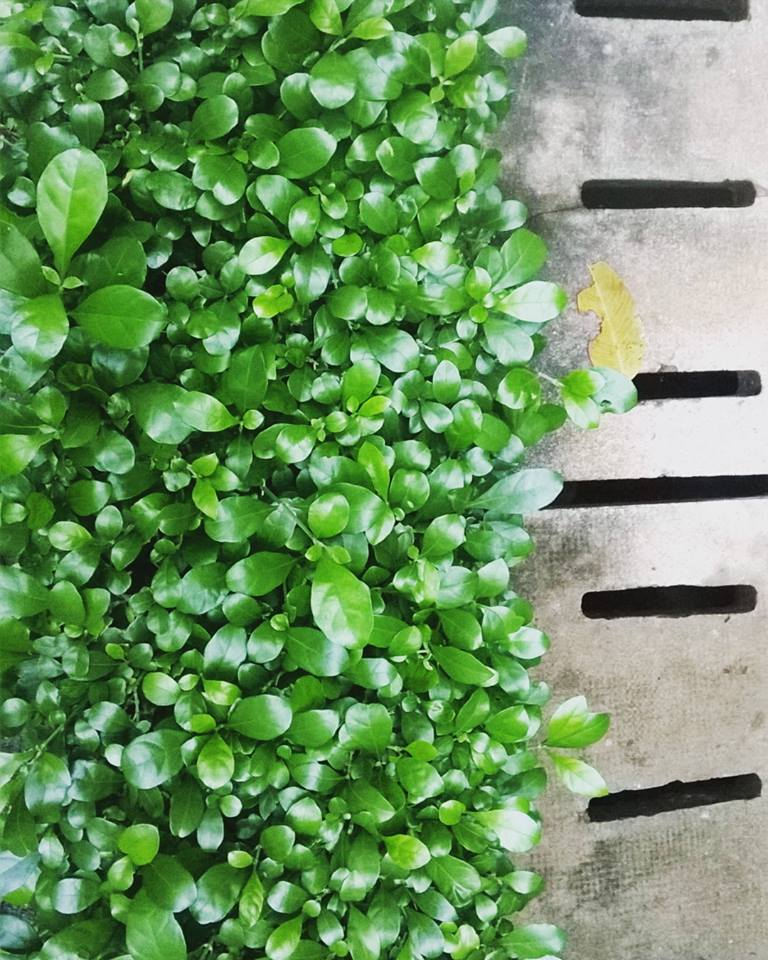
\includegraphics[width=0.8\linewidth]{C:/Users/LY/Google Drive/Git/writing_journal_article_in_rmarkdown/results/pictures/green} 

}

\caption{A green photo}\label{fig:green}
\end{figure}

\newpage

\section*{Highlights}\label{highlight}
\addcontentsline{toc}{section}{Highlights}

Short collection of bullet points: novel results + new methods\\
- submitted: separate editable file -\textgreater{} online submission
system.\\
- file name: `Highlights'\\
- 3 to 5 bullet points (maximum 85 characters, including spaces, per
bullet point)

\section*{Graphical abstract}\label{graphic}
\addcontentsline{toc}{section}{Graphical abstract}

Delete \texttt{eval=FALSE} before run the code chunk

\newpage

\section*{Cover letter}\label{cover-letter}
\addcontentsline{toc}{section}{Cover letter}

\subsubsection*{New submission}\label{new-submission}
\addcontentsline{toc}{subsubsection}{New submission}

Month Day, Year

Dear Dr.~AAA,

I am happy to submit my manuscript, \textbf{article\_name}, for your
consideration at \emph{journal\_name}. This work \emph{did sth
interesting}. The main conclusion is that \emph{sth cool}.

All of the authors have read and approved the paper and it has not been
published previously nor is it being considered by any other
peer-reviewed journal.

The manuscript has also been submitted to bioRxiv as a preprint.

Sincerely,

Author\_name, PhD\\
Professor

\subsubsection*{Resubmissions}\label{resubmissions}
\addcontentsline{toc}{subsubsection}{Resubmissions}

Month Day, Year

Dear Dr.~BBB,

I am happy to resubmit my manuscript, \textbf{article\_name}, for your
reconsideration at \emph{journal\_name}. I am grateful to you and the
reviewers who were very encouraging about the content of the
manuscript.\\
I apologize for taking so long to resubmit.\\
Too many things got in the way over the past few months.

All of the authors have read and approved the paper and it has not been
published previously nor is it being considered by any other
peer-reviewed journal.

The manuscript was previously submitted to bioRxiv as a preprint.

Sincerely,

Author\_name, PhD\\
Professor

\section*{Response to reviewers}\label{response-to-reviewers}
\addcontentsline{toc}{section}{Response to reviewers}

\subsubsection*{Reviewer \#1 (Comments for the
Author):}\label{reviewer-1-comments-for-the-author}
\addcontentsline{toc}{subsubsection}{Reviewer \#1 (Comments for the
Author):}

\textbf{copy the comment of the reviewer here}

\begin{quote}
We have revised the sentence to the following: ``sth you revised''
\end{quote}

\subsubsection*{Reviewer \#2 (Comments for the
Author):}\label{reviewer-2-comments-for-the-author}
\addcontentsline{toc}{subsubsection}{Reviewer \#2 (Comments for the
Author):}

\textbf{copy the comment of the reviewer here}

\begin{quote}
Your response here
\end{quote}

A great example
\href{https://github.com/SchlossLab/Tomkovich_PEG3350_mSphere_2021/blob/master/submission/response_to_reviewers.md}{here}.


\end{document}

